\documentclass[prb,aps,nobibnotes,twocolumn,doublespace,twocolumngrid,superbib]{revtex4}
%\documentclass[prb,aps,nobibnotes,superbib,preprint]{revtex4}

\usepackage{graphicx}
\usepackage{amsfonts}
\usepackage{amsmath}
\usepackage{bm}
\usepackage{alltt}
\usepackage{dcolumn} 
\usepackage{graphicx}
\makeatletter 
\makeatother

\begin{document}

\title{Linear scaling computation of the Fock matrix VIII. \\
       Periodic Boundary Conditions for Exact Exchange}

\author{C. J. Tymczak}
\author{Valery Weber}
\author{Eric Schwegler}
\author{Matt Challacombe}

\affiliation{Theoretical Division, Los Alamos National Laboratory, Los Alamos,
New Mexico 87545 }

\date{\today}

\begin{abstract}
We report on a consistent derivation of the exact exchange matrix for periodic
systems at the Gamma point. Previous work has always included k-space integration 
within the calculation of the exchange matrix. However, in  these methods
we can show that the calculation of the exchange matrix becomes inconsistent as the
region of k-space shrinks. This leads to a non-translation-ally invariant exchange matrix,
which is of major concern. We illustrate this problem and then show how, by a set of
simple ideas and arguments, we can retifiy it.
%
\vskip 0.07 in
\noindent{\bf Keywords}: Self-consistent-field, Exact-exchange, Linear-scaling, Gaussian-orbital 
%
\end{abstract}

\pacs{}

\maketitle

\footnotetext[1]{\tt tymczak@lanl.gov}
\footnotetext[2]{\tt vweber@lanl.gov}
\footnotetext[3]{\tt schwegler@llnl.gov}
\footnotetext[4]{\tt mchalla@lanl.gov}
\footnotetext[5]{\tt Preprint LA-UR 03-9043}


\section{INTRODUCTION}
Many calculations of the electronic structure of condensed matter systems now make use
of the exact exchange interaction 
\cite{Pisani80,REvarestov83,MCausa88,JAlmlof94,RDovesi00}. 
Whereas this has been a very
important functional in the quantum chemistry community 
\cite{PLowdin55,py,ASzabo89}, 
until the advent of the hybrid functionals 
\cite{Gill92,Becke93,ABecke96,Adamo99}, 
this functional has had very little impact on the
condensed matter electronic structure community. Now because of the accuracy obtainable with
the hybrid functionals, it has become very desirable to include exact exchange into
existing condensed matter electronic structure algorithms. 
However, most of these calculations make use of ${\bf k}$-space integrations to 
deal with the periodicity of the system \cite{RDovesi00}. However, this is not an ideal situation 
for linear scaling algorithms, where we would like to remove the need for doing
${\bf k}$-space integrations altogether by increasing the system size. 
However, when Gamma point only is attempted for exact exchange, a 
significant problem arises. For the Gamma point, in the limit of large system size,
we do not recover the ${\bf k}$-space energy per particle number; we do not have the correct
limit as particle number increases.  
%

In the proceeding sections we will first briefly review the Hartree
Foch equations of motion. Next, we will illuminate the problem that exist
for the calculation of the exchange matrix in the limit of the Gamma point for
periodic systems. We then give a solution to this problem, and then we verify that
the exchange matrix is correct in the limit of large systems as compared to a large 
${\bf k}$-space calculation done with {\bf Crystal98}. 
And finally, we verify that the exchange matrix build is indeed linear scaling
for the dense diamond system.

\section{The Hartree Fock Equations}
Within the Hatree fock approcimation we define the total energy as \cite{Pisani80,RDovesi00}
\begin{equation}
E = Tr[{\bf P} \, {\bf F}]+ E_{nn}
\label{HFEnergy}
\end{equation}
where the Fockian is defined as,
\begin{equation}
{\bf F} = 2 {\bf T}+2 {\bf V}_{en}+{\bf J}_{ee}+{\bf K}_x
\label{Fockian}
\end{equation}

\begin{eqnarray}
{\bf T}      & : & \,{\rm kinectic \, energy \, matrix} \nonumber \\
{\bf V}_{en} & : & \,{\rm electron-nuclear \, coulomb \, matrix} \nonumber \\
{\bf J}_{ee} & : & \,{\rm electron-electron \, coulomb \, matrix} \nonumber \\
{\bf K}_{x}  & : & \,{\rm exchange \, matrix} \nonumber \\
{E}_{nn}  & : & \,{\rm nuclear-nuclear \, repulsion \, energy} \nonumber \\ 
\label{Defin}
\end{eqnarray}
We solve for the density matrix, ${\bf P}$, via the eigen-equation 
\begin{equation}
{\bf F} {\bf P} = \epsilon {\bf P}
\label{DenMat}
\end{equation}
and iterate on equation (\ref{Fockian}) until self-cosistancy is reached.

\pagebreak

\section{Periodic exact exchange}

Extending methods involving local functions $\phi$ to the periodic regime, the Bloch functions
\begin{equation}
\psi^{\bf L}_c ({\bf r})
 = \sum_{\bf u}  e^{i {\bf L}\cdot{\bf u}} \phi_c ({\bf r}-{\bf u})
\label{bloch}
\end{equation}
are employed as a primary basis having the correct translational symmetry.
In Eq.~(\ref{bloch}), $\bf L$ and $\bf u$ are lattice vectors, and the sum 
formally extends over all periodic images.
To date, rapid computation of the Hartree-Fock exchange interaction demands
the analytic evaluation of two-electron integrals, which is possible when the 
local basis functions are of Cartesian Gaussian type.  Typically, these functions have the form
\begin{equation}
\phi_c ({\bf r}) = (x-C_x)^{l_c} (y-C_y)^{m_c} (z-C_z)^{n_c}{\large e}^{-\zeta_c ({\bf r}-{\bf C})^2}
\end{equation}
where $\bf C$ is an atom center, the triad $\{l_c,m_c,n_c\}$ sets angular symmetry  
and the exponent $\zeta_c$ is chosen to describe a 
particular length scale. Gaussian basis functions are often contracted to approximate 
atomic eigenfunctions \cite{}.
 
With periodic boundary conditions, the exact Hartree-Fock exchange matrix is \cite{MCausa88}
\begin{equation}
K^{\bf M}_{ab}= - \frac{1}{2}
\sum _{{\bf L N} c d} P^{\bf L}_{cd}
\left(
      \psi        _a    
      \psi^{\bf L}_c    
{\big | }
      \psi^{\bf M}_b    
      \psi^{\bf N+L}_d  
\right)
\label{CryEq}
\end{equation}
where the two-electron integrals have been written in chemists notation:
\begin{eqnarray}
\lefteqn{
\left(
      \psi        _a  
      \psi^{\bf L}_c  
{\big | }
      \psi^{\bf M}_b  
      \psi^{\bf N+L}_d
\right)
= }  \nonumber \\
&& \qquad\qquad
\iint d {\bf r} d {\bf r}'
      \frac{
      \psi        _a    ({\bf r}) 
      \psi^{\bf L}_c    ({\bf r})~ 
      \psi^{\bf M}_b    ({\bf r'})
      \psi^{\bf N+L}_d  ({\bf r'})}
      {\left|{\bf r}-{\bf r'}\right|} .
\end{eqnarray}

The formally infinite sums over lattice vectors in Eq.~(\ref{CryEq}) involve 
many contributions that are in practice infinitesimal.  In part this is due to 
the decay between local basis function products $\phi_a \phi_c $; the product of
two Guassians centered at $\bf A$ and $\bf C$ decays also as a Gaussian with $|{\bf A}-{\bf C}|$. 
Truncation based purely on the overlap of Gaussian basis functions is reliable and
well controlled, leading efficiently to ${\cal O}(N)$ product terms.
Additionally, the density matrix is known to decay exponentially 
for non-metalic systems.  A radial cutoff $r_x$ defining the range of allowed exchange 
interactions may be used to exploit this fall off {\em a priori} by confining summation over 
$\bf L$ and ${\bf M}$ \cite{REuwema74,CPisani80,RDovesi80,MCausa88} to only those terms that 
satisfy the imposed geometric contraints.  Radial cutoffs are also used to achieve
$N$-scaling of the exchange matrix in gas phase calculations by limiting the allowed range 
of atom centers $\bf C$ and $\bf D$ corresponding to matrix elements $P_{cd}$\cite{}.  

\pagebreak
These schemes have been implimented in the
{\em ab initio} program CRYSTAL \cite{}, allowing the routine calculation of periodic systems
with the HF and HF/DFT model chemistries.

\section{Exchange at the $\Gamma$-point}

The $\Gamma$-point approximation lifts translational invarience of the Bloch functions, limiting
$\bf k$-space sampling to just the central cell; 
 $\psi^{\bf k}_c \rightarrow \delta_{\bf k,0} \sum_{\bf u} \phi_c ({\bf r}-{\bf u})$.
With $N$-scaling algorithm, the effects of $\bf k$-space integration may be recouped 
with increasing cell-size.  In this approximation, Eq.~(\ref{CryEq}) reduces to 
\begin{equation}
K_{ab}=
\sum _{{\bf u v} c d} P_{cd}
\left(
      \phi        _a    
      \phi^{\bf u}_c    
{\big | }
      \phi        _b    
      \phi^{\bf v}_d  
\right)
\label{CryEq}
\end{equation}

However, in this approximation the exact exchange potential, symmetric in the limit of infinite 
summation, has been asymetically truncated, resulting in a potential that depends on position 
of the unit cell.  Translational invarience can be restored to the exchange $\Gamma$-point approximation 
by imposing the minimum image criterion (MIC) to the exchange interaction:
\begin{equation}
K_{ab}=
\sum _{{\bf u v} c d} P_{cd}
\left(
      \phi        _a    
      \phi^{\bf u}_c    
{\big | }
      \phi        _b    
      \phi^{\bf v}_d  
\right)_{\rm  MIC}.
\label{MIC}
\end{equation}
This criterion is applied at the contraction phase, ensuring that primitive charge distributions 
interact consistently over a minimum distance.  In particular, if the primitive basis 
function product $\phi_a \phi^{\bf u}_c$ is centered at $\bf P$ and the primitive product 
$\phi_b \phi^{\bf v}_d$ is at $\bf Q$, then the minimum image criterion is 
applied simply to the interaction vector $ {\bf P}-{\bf Q} $
\begin{verbatim}
FPQx=PQx*InvBox(1,1)+PQy*InvBox(1,2)+PQz*InvBox(1,3)
FPQy=PQy*InvBox(2,2)+PQz*InvBox(2,3)
FPQz=PQz*InvBox(3,3)
FPQx=FPQx-ANINT(FPQx)
FPQy=FPQy-ANINT(FPQy)
FPQz=FPQz-ANINT(FPQz)
PQx =FPQx*Box(1,1)+FPQy*Box(1,2)+FPQz*Box(1,3)
PQy =FPQy*Box(2,2)+FPQz*Box(2,3)
PQz =FPQz*Box(3,3)
\end{verbatim}
where {\tt Box} is the box shape of the unit cell and {\tt InvBox} are the inverse lattice vectors.
{\bf CJ, we could use one sentance describing what this code does;  changes to fractionals, wraps? back transforms...}.
This approach is completely general, and can be used at the primitive level with any modern approach
to computing two-electron integrals. 

Suprisingly, this work is the first to correctly define the exact Hartree-Fock 
exchange potential for periodic boundary conditions and the $\Gamma$-point approximation.  Moreover,
effects related to asymetric truncation may also manifest in methods that perform incomplete $\bf k$-space 
sampling, and may benifit from employing the minimum image criterion. 

\pagebreak

\section{Implimentation}

A general treatment of $\Gamma$-point Periodic Boundary Conditions has been implimented in the MondoSCF
suite of programs for linear scaling programs quantum chemistry.  The program {\sc ONX} \cite{} has been 
modified by straighforwardly performing double loops over the lattice vectors $\bf v$ and $\bf u$
arround the original ONX loop structure \cite{}.  Thus, ordered bra and ket distribution buffers are 
assembled for each lattice vector pair.   Also the symmetry driven Head-Gordon Pople scheme for 
computing two-electron integrals, innermost to the ONX loops, has been modified to include the 
minimum image criterion in the contraction stage of the Vertical Recurence Relations.  While this implimentation
is linear scaling and simple, it suffers from a number of drawbacks that we will set forth in detail shortly, 
together with a more efficient algorithm able to achieve scalable parallelism \cite{}.

\pagebreak

\begin{table}
\caption{Comparison \textbf{MondoSCF} and \textbf{Crystal98} for a 
Magnesium Oxide test system within the Hartree-Fock approxiamtion using
the STO-3G basis set. The \textbf{MondoSCF} calculations where done to
the accuracy of the quoted digits. All calculations where done at the Gamma point
for comparison except the last \textbf{Crystal98} calculation, which was done at 
${\bf k}_{max}=\{6,6,6\}$.}
\label{table:ComToCrystal98}
\begin{tabular}{crll}
\toprule
Program         & $N_{\rm at}$              & Energy (au)   & Energy/$N_{\rm at}$\\ 
\colrule
{\sc MondoSCF}       & 8$^g$    & -1098.4382  & -137.30478 \\
     --              & 16$^f$   & -2197.0564  & -137.31603 \\
     --              & 32$^g$   & -4394.4846  & -137.32764 \\
{\sc Crystal98}$^h$  & 32$^g$   & -4394.5847  & -137.33077 \\
{\sc MondoSCF}       & 54$^f$   & -7415.8962  & -137.33141  \\
     --              & 64$^g$   & -8789.2494  & -137.33202  \\
{\sc Crystal98}$^h$  & 64$^g$   & -8789.2484  & -137.33201 \\
{\sc MondoSCF}       & 128$^f$  & -17578.502  & -137.33205 \\
     --              & 216$^g$  & -29663.729  & -137.33208 \\ 
\hline
{\sc Crystal98}$^i$  & 2\       & -274.66415  & -137.33208  \\ 
\botrule 
\end{tabular}

$^f$Triclinic~~
$^g$Cubic~~
$^h$Gamma Point \\
$^i 8\times8\times8$ $\bf k$-space grid  \\
\end{table}


\begin{table}
\caption{Comparison \textbf{MondoSCF} and \textbf{Crystal98} for a proton ordered ice
test system within the Hartree-Fock approxiamtion using
a crystal optimized basis set\cite{CBS:511G:H,CBS:861G:MgO}. 
The \textbf{MondoSCF} calculations where done to
the accuracy of the quoted digits. All calculations where done at the Gamma point
for comparison except the last \textbf{Crystal98} calculation, which was done at 
${\bf k}_{max}=\{6,6,6\}$.}
\label{table:ComToCrystal98_Ice}
\center{
\begin{tabular}{lrll}
\toprule
{\sc MondoSCF}  & 2$^a$    &  -152.03025  &  -76.01512 \\
                & 16$^a$   &  -1216.3003  &  -76.01877 \\
                & 54$^a$   &  -4105.0163  &  -76.01882 \\
                & 128$^a$  &  -9730.4090  &  -76.01882 \\
                & 250$^a$  &  -19004.705  &  -76.01882 \\ 
\hline
{\sc Crystal98}$^b$  & 2   &  -152.03765  &  -76.01882   \\ 
\botrule
\multicolumn{4}{l}{$ ^a $Gamma Point.} \\
\multicolumn{4}{l}{$ ^b 6\times6\times6$ $k$-space grid.}
\end{tabular}}
\end{table}



\section{Results}

Table \ref{table:ComToCrystal98} shows our results for the total
energy for Magnesium Oxide as compared to results obtained from \textbf{Crystal98}.
for the STO-3G basis set for increasing system size. We see that we obtain excellent
convergence to the {\bf Crystal98} large ${\bf k}$-space calculation. This verifies that
our methodology for doing the exchange matrix at the Gamma point is correct, and converges 
in the correct fashion in regard to increasing system size. In table \ref{table:ComToCrystal98_Ice}
we show the convergence of the proton ordered ice system as compared to results obtained from 
\textbf{Crystal98} using a more accurate crystal optimized basis set. Again we see excellent
agreement with the \textbf{Crystal98} results.


\section{Scaling}
 
Figure \ref{figure:Scaling_Matrix_Build} is the time it takes to build the
exact exchange matrix  \( K_{x} \) for the periodic diamond system up to 800 atoms for the modified pople 
basis set 6-31G$ ^\dagger$ \cite{Pople92} and for a matrix thresholding of $\tau=10^{-3}$ .
Also included in the figure for comparision are the total time for the
density matrix solver, TRS4 \cite{ANiklasson03}, 
and the Coulomb matrix build using our Quantum chemical treee code \cite{CTymczak03c}. 


\ref{figure:EnergyVsLattice}
%We also show in figure \ref{figure:EnergyPerN} the energy per carbon atom and 
%in figure \ref{figure:ErrorPerN} the relative error in the total energy. 
%Again we see the convergence of the total energy
%as a function of increasing system size, which is akin to k-space integration.
%We also see that our relative error is very well controlled within the \
%textbf{MondoSCF} quantum chemistry code, even up to 512 carbon atoms.


\section{CONCLUSIONS}
We have shown a consistent derivation for the exact exchange integrals at the $\Gamma$-point. 

\section*{ACKNOWLEDGMENTS}

We would like to acknowledge Tommy Sewell and Ed Kober for there advise
and support. We would also like to thank Anders Niklasson for his help
in preparation of this manuscript. 

\bibliographystyle{apsrmp} 
\bibliography{mondo_new} 


%
%
%
%
%
\begin{figure}
\caption{Unit cell and its brava lattice vectors.}
\label{figure:SimCell}
{\centering \includegraphics{UnitCell_2.ps} \par}
\end{figure}
%
%
%
\begin{figure}
\caption{For the Gamma point, the region in which atom $a$ has exchange interactions.}
\label{figure:ExchangeRegion}
{\centering \includegraphics{ExchangeRegion.ps} \par}
\end{figure}
%
%
%
\begin{figure}
\caption{For ${\bf k}_{max}=\{1,1,1\}$, the region in which atom $a$ has exchange interactions.}
\label{figure:ExchangeRegion_k111}
{\centering \includegraphics{ExchangeRegion_k111.ps} \par}
\end{figure}
%
%
%
\begin{figure}
\caption{Scaling results for the exchange matrix build, the coulomb matrix
build (scaled by ten), and the density matrix solver (scaled by twenty),  
for the dense diamond periodic system up to 800 atoms using the
6-31G$ ^\dagger$ basis set.}
\label{figure:Scaling_Matrix_Build}
{\centering \includegraphics{Timing_Diamond_ONX.ps} \par} 
\end{figure}
%
%
%
\begin{figure}
\caption{Energy per Carbon atoms vs. Lattice constants for a {\bf Crystal98} calculation 
with a two atoms per unit
cell and ${\bf k}_{max} = (12,12,12)$, a {\bf MondoSCF} calculation with 64 atoms per
unit cell at the Gamma-point at a tight level of accuracy, and a {\bf MondoSCF} calculation 
with 512 atoms  per
unit cell at the Gamma-point at a loose level of accuracy.
All calculation where done using the 
6-31G$ ^\dagger$ basis set hartree fock theory level. }
\label{figure:EnergyVsLattice}
{\centering \includegraphics{Diamond_En_vs_V.ps} \par} 
\end{figure}
%
%
%
\begin{figure}
\caption{Scaling results for the exchange matrix build, coulomb matrix
build and the density matrix solver  for the proton ordered ice periodic system up to 432 water molecules 
using a crystal optimized basis set\cite{CBS:511G:H,CBS:861G:MgO} for a matrix threshold of $\tau=10^{-4}$.}
\label{figure:Scaling_Matrix_Build_Ice}
{\centering \includegraphics{Timing_pIce_ONX_1.ps} \par} 
\end{figure}
%
%
%
\begin{figure}
\caption{Scaling results for the exchange matrix
build  for the proton ordered ice periodic system up to 432 water molecules 
using a crystal optimized basis set\cite{CBS:511G:H,CBS:861G:MgO} for a matrix threshold of 
$\tau=10^{-4}$ and  $\tau=10^{-6}$.}
\label{figure:Scaling_Matrix_Build_Ice}
{\centering \includegraphics{Timing_pIce_ONX_2.ps} \par} 
\end{figure}
%
%
%
\begin{figure}
\caption{Energy per Molecule vs. the $a_0$ Lattice constans for a {\bf Crystal98} calculation 
with a two molecules per unit cell and ${\bf k}_{max} = (6,6,6)$ and a {\bf MondoSCF} calculation 
with 432 molecules  per unit cell at the Gamma-point at a loose level of accuracy.
All calculation where done using a crystal optimized basis set\cite{CBS:511G:H,CBS:861G:MgO} 
hartree fock theory level. }
\label{figure:EnergyVsLattice_Ice}
{\centering \includegraphics{pIce_En_vs_a.ps} \par} 
\end{figure}
%
%
%
%
\end{document}
